%!TEX TS-program = xelatex
\documentclass[12pt, a4paper, oneside]{article}

\usepackage{amsmath,amsfonts,amssymb,amsthm,mathtools}  % пакеты для математики

\usepackage[english, russian]{babel} % выбор языка для документа
\usepackage[utf8]{inputenc} % задание utf8 кодировки исходного tex файла
\usepackage[X2,T2A]{fontenc}        % кодировка

\usepackage{fontspec}         % пакет для подгрузки шрифтов
\setmainfont{Linux Libertine O}   % задаёт основной шрифт документа

\usepackage{unicode-math}     % пакет для установки математического шрифта
\setmathfont[math-style=upright]{Neo Euler} % шрифт для математики

% Конкретный символ из конкретного шрифта
% \setmathfont[range=\int]{Neo Euler}

%%%%%%%%%% Работа с картинками %%%%%%%%%
\usepackage{graphicx}                  % Для вставки рисунков
\usepackage{graphics}
\graphicspath{{images/}{pictures/}}    % можно указать папки с картинками
\usepackage{wrapfig}                   % Обтекание рисунков и таблиц текстом

%%%%%%%%%%%%%%%%%%%%%%%% Графики и рисование %%%%%%%%%%%%%%%%%%%%%%%%%%%%%%%%%
\usepackage{tikz, pgfplots}  % язык для рисования графики из latex'a

%%%%%%%%%% Гиперссылки %%%%%%%%%%
\usepackage{xcolor}              % разные цвета

\usepackage{hyperref}
\hypersetup{
	unicode=true,           % позволяет использовать юникодные символы
	colorlinks=true,       	% true - цветные ссылки, false - ссылки в рамках
	urlcolor=blue,          % цвет ссылки на url
	linkcolor=red,          % внутренние ссылки
	citecolor=green,        % на библиографию
	pdfnewwindow=true,      % при щелчке в pdf на ссылку откроется новый pdf
	breaklinks              % если ссылка не умещается в одну строку, разбивать ли ее на две части?
}


\usepackage{todonotes} % для вставки в документ заметок о том, что осталось сделать
% \todo{Здесь надо коэффициенты исправить}
% \missingfigure{Здесь будет Последний день Помпеи}
% \listoftodos --- печатает все поставленные \todo'шки

\usepackage[paper=a4paper, top=20mm, bottom=15mm,left=20mm,right=15mm]{geometry}
\usepackage{indentfirst}       % установка отступа в первом абзаце главы

\usepackage{setspace}
\setstretch{1.15}  % Межстрочный интервал
\setlength{\parskip}{4mm}   % Расстояние между абзацами
% Разные длины в латехе https://en.wikibooks.org/wiki/LaTeX/Lengths


\usepackage{xcolor} % Enabling mixing colors and color's call by 'svgnames'

\definecolor{MyColor1}{rgb}{0.2,0.4,0.6} %mix personal color
\newcommand{\textb}{\color{Black} \usefont{OT1}{lmss}{m}{n}}
\newcommand{\blue}{\color{MyColor1} \usefont{OT1}{lmss}{m}{n}}
\newcommand{\blueb}{\color{MyColor1} \usefont{OT1}{lmss}{b}{n}}
\newcommand{\red}{\color{LightCoral} \usefont{OT1}{lmss}{m}{n}}
\newcommand{\green}{\color{Turquoise} \usefont{OT1}{lmss}{m}{n}}

\usepackage{titlesec}
\usepackage{sectsty}
%%%%%%%%%%%%%%%%%%%%%%%%
%set section/subsections HEADINGS font and color
\sectionfont{\color{MyColor1}}  % sets colour of sections
\subsectionfont{\color{MyColor1}}  % sets colour of sections

%set section enumerator to arabic number (see footnotes markings alternatives)
\renewcommand\thesection{\arabic{section}.} %define sections numbering
\renewcommand\thesubsection{\thesection\arabic{subsection}} %subsec.num.

%define new section style
\newcommand{\mysection}{
	\titleformat{\section} [runin] {\usefont{OT1}{lmss}{b}{n}\color{MyColor1}} 
	{\thesection} {3pt} {} } 


%	CAPTIONS
\usepackage{caption}
\usepackage{subcaption}
%%%%%%%%%%%%%%%%%%%%%%%%
\captionsetup[figure]{labelfont={color=Turquoise}}

\pagestyle{empty}

%%%%%%%%%% Свои команды %%%%%%%%%%
\usepackage{etoolbox}    % логические операторы для своих макросов

% Все свои команды лучше всего определять не по ходу текста, как это сделано в этом документе, а в преамбуле!

% Одно из применений - уничтожение какого-то куска текста!
\newbool{answers}
\booltrue{answers}
%\boolfalse{answers}

\usepackage{enumitem}
% бульпоинты в списках
\definecolor{myblue}{rgb}{0, 0.45, 0.70}
\newcommand*{\MyPoint}{\tikz \draw [baseline, fill=myblue,draw=blue] circle (2.5pt);}
\renewcommand{\labelitemi}{\MyPoint}

% расстояние в списках
\setlist[itemize]{parsep=0.4em,itemsep=0em,topsep=0ex}
\setlist[enumerate]{parsep=0.4em,itemsep=0em,topsep=0ex}


\begin{document}
	
\section*{Семинар 6: Логистическая регрессия}

\subsection*{И не задача вовсе, а подводка}

Давайте построим логистическую регрессию также как мы сделали это на семинаре.  До этого мы с вами уже имели дело с обычной регрессией: 

$$
y = \beta_0 + \beta_1 \cdot x.
$$

Когда мы оценивали её, мы рисовали через облако точек линию: 

\begin{center}
	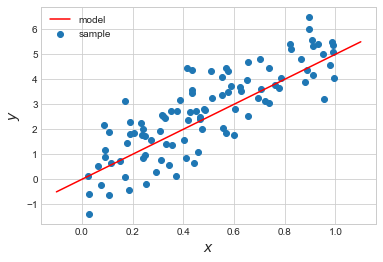
\includegraphics[scale=0.7]{regr.png}
\end{center}

Переменная, которую мы прогнозировали, $y$, принимала любые значения и всё было хорошо. Теперь мы решаем задачу классификации. Наша переменная принимает значения либо $0$ либо $1$. Если мы опять будем строить обычную регрессию, мы попадём в глупую ситуацию: 

\begin{center}
	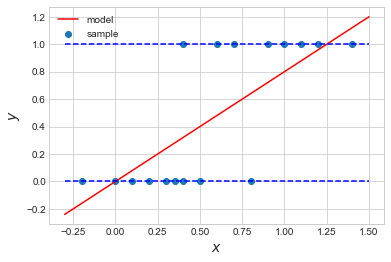
\includegraphics[scale=0.7]{logreg_problem.png}
\end{center}

Наша голубая линия регрессии снова пройдёт через облако точек. Когда мы будем пытаться на её основе построить прогноз, мы будем получать абсолютно любые значения. Это могут быть и $-7$, и $2.1$, и $1$, и даже $0.33$.  

В принципе, мы можем интерпретировать эти числа как уверенность нашей модели. Например, если получилось $55$, значит модель уверена в том, что класс первый. А если получилось $-33$, модель уверена, что класс нулевой. Ну а если $0.5$, то модель колеблется. 

Правда эту степень уверенности хорошо было бы пронормировать. Обычно это делают на отрезок от нуля до единицы. Для этого вместо линии рисуют вот такую $S$-образную  кривую: 

\begin{center}
	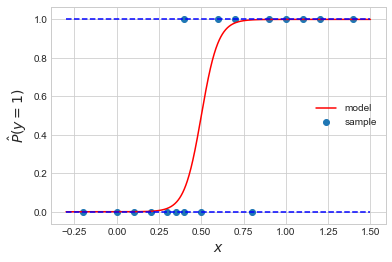
\includegraphics[scale=0.7]{logreg_solveprob.png}
\end{center}

Тогда значения принимаются на отрезке от $0$ до $1$ и мы можем их интерпретировать как вероятность первого класса, $P(y = 1)$. Какую функцию можно взять для такой кривой? Из теории вероятностей вы знаете, что все функции распределения ведут себя $S$-образно.  В машинном обучении обычно берут логичтическую функцию распределения, потому что она очень простая: 

$$
P(y = 1) = \frac{1}{1 + e^{-z}}.
$$

Такую функцию иногда называют сигмоидой. Так и получается логичтическая регрессия. На первом шаге мы считаем "уверенность" модели: 

$$
z = \beta_0 + \beta_1 \cdot z,
$$

а на втором шаге превращаем её в вероятность с помощью сигмоиды.  Из-за того, что мы используем логистическое распределение, такую регрессию называют логистической.  

Модель построена. Дело осталось за малым. Выбрать функцию потерь. В случае регрессии мы использовали с вами $MSE$. В случае логистической регрессии мы также можем попробовать использовать его же, но нам бы хотелось придумать что-то новое. Новая функция потерь должна подходить для нашей задачи по смыслу.

Наши $y$ могут принимать значения $1$ и $0$. Если $y = 1$, мы хотим, чтобы модель спрогнозировала $\hat p = P(y= 1)$ побольше.  Если $y = 0$, мы хотим, чтобы модель спрогнозировала $\hat p$ поменьше, то есть $ 1 - \hat p$ побольше. 

Тогда мы можем выписать такую штуку: 

$$
-1 \cdot (y \cdot \hat p  + (1 - y) (1 - \hat p)).
$$

Нам надо найти её минимум по $\beta$. Тогда модель будет работать хорошо. Если $y = 1$, мы будем получать большое $\hat p$, так ка второе слагаемое в нашей формуле будет зануляться. Если $y = 0$, то будет зануляться первое слагаемое, и мы будем пытаться получить большое $1 - \hat p$. 

Функция потерь почти готова. Остался последний штрих.  Давайте заставим нашу функцию штрафовать нас при сильных ошибках сильнее, как это было в случае $MSE$ для регрессии. Для этого нужно взять от $\hat p$ логарифм и получить: 

$$
-1 \cdot (y \cdot \ln \hat p  + (1 - y)  \ln (1 - \hat p)).
$$

Это будет наша итоговая функция потерь. Она называется logloss и обычно используется для обучения логистической регрессии. 

Остаётся только одни вопрос: почему логарифм вносит более большой штраф для более сильных ошибок.  Давайте нарисуем $\ln \hat p$ и $\ln (1 - \hat p)$ на картинке\footnote{{\color{blue} \url{https://dyakonov.org/2018/03/12}}}.


\begin{center}
	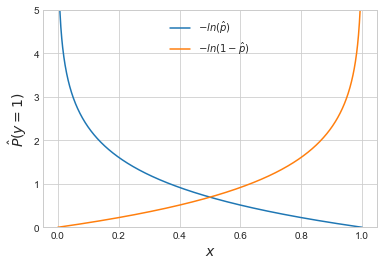
\includegraphics[scale=0.7]{log_loss_05.png}
\end{center}


Когда $y=1$ мы пытаемся сделать поменьше $- \ln \hat p$. Если он оказался очень большим, надо делать его меньше существенно сильнее, если он уже итак маленький. Посмотрите на синюю кривую. Это наш логарифм. Поначалу он убывает очень резко, а после медленнее. Это позволяет штрафовать за сильные ошибки сильнее. 

И практически никакой математики. Одна сплошная интуиция. На самом деле ровно такую же функцию потерь можно получить без интуиции. Вы этим займётесь на математической статистике, когда будете изучать метод максимального правдоподобия. Попробуйте ради интереса в будущем вернуться к логистической регрессии и вывести функцию потерь. 



\subsection*{Задача 1}

Винни Пух (ВП) --- исследователь и пасечник. Пчёлы ВП откладывают мёд. ВП пробует его и понимает, правильной оказалась пчела или нет. Спустя многие годы работы ВП накопил довольно большую выборку из правильных и неправильных пчёл и смог на основе неё оценить модель: 

$$ 
z = 1 + 0.5 \cdot x,
$$

где $x$ --- это количество мёда, которое снесла пчела.  Предположим, что ВП сталкивается с новой пчелой. Он знает, что она снесла $x = 6$ килограмм мёда. Какова вероятность того, что эта пчела правильная? Предположим, что эта пчела оказалась неправильной. Какой logloss совершает ВП? Какой logloss будет, если эта пчела оказалась правильной? 

\ifbool{answers}{
	\textbf{Решение:}

Найдём "уверенность" ВП в правильности пчелы: 

$$
z  =  1 + 0.5 \cdot 6  = 4.
$$

Превратим её в вероятность с помощью сигмоиды: 

$$
\hat P(y  = 1) = \frac{1}{1 + e^{-z}} = \frac{1}{1 + e^{-4}} = 0.98.
$$

Получаем, что вероятность того, что пчела правильная $0.98$. Пусть эта пчела в реальности оказалась правильной. Найдём для неё logloss: 

$$
-1 \cdot (1 \cdot \ln 0.98 + (1 - 1) \cdot \ln (1 - 0.98)) = 0.021.
$$

За ошибку отвечает первое слагаемое. Вероятность того, что пчела была правильной оказалась довольно высокой. Пчела и правда оказалась правильной. Однако вероятность была чуть меньше единицы. Мы не были абсолютно уверены, а значит немного ошибались. logloss формализует это "немного" в виде числа. 

Теперь найдём logloss в случае, если пчела в реальности оказалась неправильной. Тут за ошибку отвечает второе слагаемое. Мы, сказав что вероятность её правильности $0.98$ очень сильно ошиблись. Посмотрим каким станет logloss: 

$$
-1 \cdot (0 \cdot \ln 0.98 + (1 - 0) \cdot \ln (1 - 0.98)) = 4.1.
$$

Ошибка довольно сильно выросла.
}


\subsection*{Задача 2}

У ВП в тестовой выборке есть две пчелы. Одна правильная, одна неправильная.  Он хочет проверить на этой выборке свою модель. Она предсказала, что первая правильная с вероятностью $0.6$, а вторая с вероятностью $0.4$. Найдите средний logloss на этой выборке. 

\ifbool{answers}{
	\textbf{Решение:}

\begin{equation*}
\begin{aligned}
logloss = -\frac{1}{2} \cdot (  & (1 \cdot \ln(0.6) + (1 - 1) \cdot \ln(1 - 0.6)) + \\
                                               & (0 \cdot \ln(0.4) + (1 - 0) \cdot \ln(1 - 0.4))) = \\
                                               & -0.5 \cdot (\ln 0.6 + \ln 0.6) = -\ln 0.6 \approx  0.51
\end{aligned}
\end{equation*}

}


\subsection*{Задача 3}

ВП построил для своей выборки картинку, чтобы посмотреть насколько его выборка сбалансированна. Получилось вот так: 

\begin{center}
	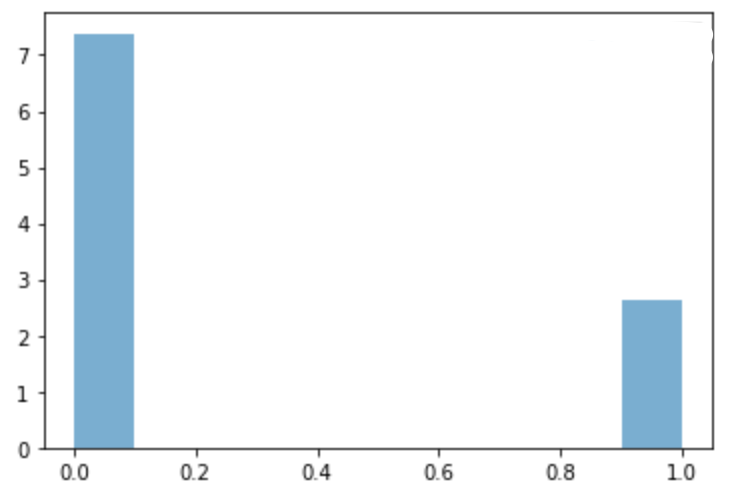
\includegraphics[scale=0.25]{balance_logloss.png}
\end{center}

Обычно ВП минимизировал такой logloss: 

$$
- \frac{1}{n} \sum_{i=1}^n (y_i \cdot \ln \hat p_i + (1 - y_i) \cdot \ln( 1 - \hat p_i)) 
$$

В этот раз ВП решил минимизировать немного модернизированную функцию: 

$$
- \frac{1}{n} \sum_{i=1}^n ({\color{red} 3 \cdot} y_i \cdot \ln \hat p_i + {\color{red} 1 \cdot} (1 - y_i) \cdot \ln( 1 - \hat p_i)) 
$$

Как думаете, зачем ВП сделал это? 

\ifbool{answers}{
	\textbf{Решение:}

ВП увидел, что в выборке есть серьёзный дисбаланс. Первый класс встречается в три раза реэе нулевого.  Из-за этого ВП решил искусственно увеличить значение каждого слагаемого с $\ln \hat p_i$ для первого класса в три раза. Если хочется сделать такое в \textbf{sklearn}, можно внутри \textbf{LogisticRegression} поставить \textbf{weighted = 'balanced'}. Тогда он сам рассчитает насколько велик дисбаланс в тренировочной выборке и увеличит одно из слагаемых. 
}


\subsection*{Задача 4 (для настоящих дата саунистов)}

\textbf{Задачка со звёздочкой. Для тех, кто интересуется. Её не будет в самостоялке! Несмотря на это она довольно простая.} На семинаре мы сказали, что логистическую регрессию тоже можно учить с помощью градиентного спуска. Давайте попробуем сделать один шаг этой процедуры. 

У ВП есть логистическая регрессия и функция потерь: 

\begin{equation*}
\begin{aligned}
&z  = \beta \cdot x \\
&P(y = 1) = \frac{1}{1 + e^{-z}} \\
&logloss = -1 (y \cdot \ln \hat p + (1 - y) \cdot \ln (1 - p))
\end{aligned}
\end{equation*}

Оказалось, что $x = -5$, а $y = 1$. Сделайте один шаг градиентного спуска, если $\beta_0 = 1$, а скорость обучения $\gamma = 0.01$. 


\ifbool{answers}{
	\textbf{Решение:}
	
Сначала нам надо найти $logloss'_{\beta}$. В принципе в этом и заключается вся сложность задачки. Давайте подстави вместо $\hat p $ в logloss сигмоиду. 

$$
logloss = -1 \left (y \cdot \ln \left( \frac{1}{1 + e^{-z}} \right)  + (1 - y) \cdot \ln \left ( 1 - \frac{1}{1 + e^{-z}} \right ) \right)
$$
	
Теперь подставим вместо $z$ уравнение регрессии:
	

$$
logloss = -1 \left (y \cdot \ln \left( \frac{1}{1 + e^{-\beta \cdot x}} \right)  + (1 - y) \cdot \ln \left ( 1 - \frac{1}{1 + e^{- \beta \cdot x}} \right ) \right)
$$

Это и есть наша функция потерь.  От неё нам нужно найти производную. Давайте подготовимся. Делай раз, найдём производную $logloss$ по $\hat p$: 

$$
logloss'_{\hat p} = -1 \left(y \cdot \frac{1}{\hat p} - (1 - y) \cdot \frac{1}{(1 - p)} \right)
$$

Делай два, найдём производную $\frac{1}{1 + e^{-\beta x}} $ по $\beta$: 

\begin{multline*}
\left(  \frac{1}{1 + e^{-\beta x}}   \right)'_{\beta}  = - \frac{1}{(1 + e^{-\beta x})^2} \cdot e^{-\beta x} \cdot (-x) =\frac{1}{1 + e^{-\beta x}}  \cdot \frac{e^{-\beta x}}{1 + e^{-\beta x}} \cdot x  = \\ = \frac{1}{1 + e^{-\beta x}}  \cdot  \left(1 - \frac{1}{1 + e^{-\beta x}}  \right) \cdot x
\end{multline*}

По-другому это можно записать как $\hat p \cdot (1 - \hat p) \cdot x$.  \textbf{Всё.} Давайте искать полную производную:

\begin{multline*}
logloss'_{\beta} = -1 \left(y \cdot \frac{1}{\hat p}  \cdot  \hat p \cdot  \left(1 - \hat p)  \right) \cdot x  - (1 - y) \cdot \frac{1}{(1 - \hat p)} \cdot  \hat p \cdot  \left(1 - \hat p)  \right) \cdot x \right) = \\ =  -y \cdot \left( 1 - \hat p \right) \cdot x + (1 - y) \cdot  \hat p  \cdot x =  (-y + y \hat p  + \hat p - y \hat p ) \cdot x = (\hat p - y) \cdot x
\end{multline*}
	
Найдём значение производной в точке $\beta_0 = 1$ для нашего наблюдения $x = -5, y=1$: 

$$
\left(\frac{1}{1 + e^{-1 \cdot (-5)}}  - 1 \right) \cdot (-5)  \approx  4.96
$$

Делаем шаг градиентного спуска: 

$$
\beta_1 = 1 - 0.01 \cdot 4.96 \approx 0.95
$$		

}


\end{document}
